\chapter{RC 5}
\recitation{5}{3 Nov. 18:30}{}

\section{Laws of large number}
Congratulation! You have made it to this chapter. The tools we are going to learn in this chapter is more structured compare to the previous ones. 
We start with Markov inequality and end with the weak law of large number. To give rough structure
\[
    \text{Markov inequality} \implies \text{Chebyshev inequality} \implies \text{WLLN}  
\]

\subsection{Some inequalities}
Although we don't use it directly, union bound is quite useful.
\begin{note}[Union bound]
   For any events \(A_1, \dots, A_n\),
   \[
    P(\cup_{i =1}^n A_i) \leq  \sum_{i=1}^{n} P(A_i)
   \]  
\end{note}
\subsubsection*{Markov inequality}
Markov inequality give the \textbf{tail bound} of the nonnegative random variable.  
\begin{note}[Markov inequality]
    Let X be a \textbf{nonnegative} r.v.  Then, for any \(t > 0\)
    \[
        P(X \geq  t) \leq \frac{E[X]}{t}
    \] 
\end{note}
There are many approach to get Markov inequality, it is worthwhile to check them out. 
Before you do so, I would like to introduce a application of Markov inequality in communication technology. 
\subsubsection*{BPSK}
(Skipping this won't hurt your understanding of this chapter and will not be on any test.)\\ 
\begin{figure*}[hbt]
    \centering
    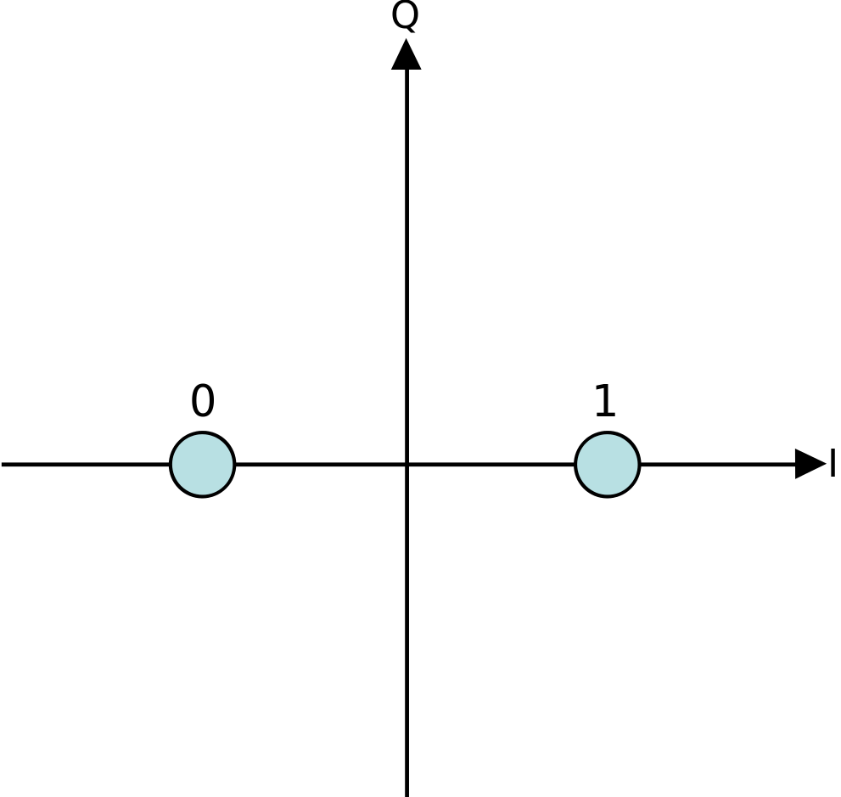
\includegraphics[width=0.25\textwidth]{./Figures/Constellation.png}
    \caption*{Picture in the wiki page. BPSK symbol.}
\end{figure*}
\textbf{Abstraction}\\
Binary in BPSK means that in each round of transmission, \textbf{transmitter} either send \(-\sqrt{E_0}\) or \(\sqrt{E_0}\), where \(E_0\) is the transmitting energy. 
However, there will be some noise real world, and we usually take the noise as a Gaussian random variable \(w\) follows N(0, \(\frac{N_0}{2}\) ) (It is okay we will use a graph to show this). 
\begin{figure*}[hbt]
    \centering
    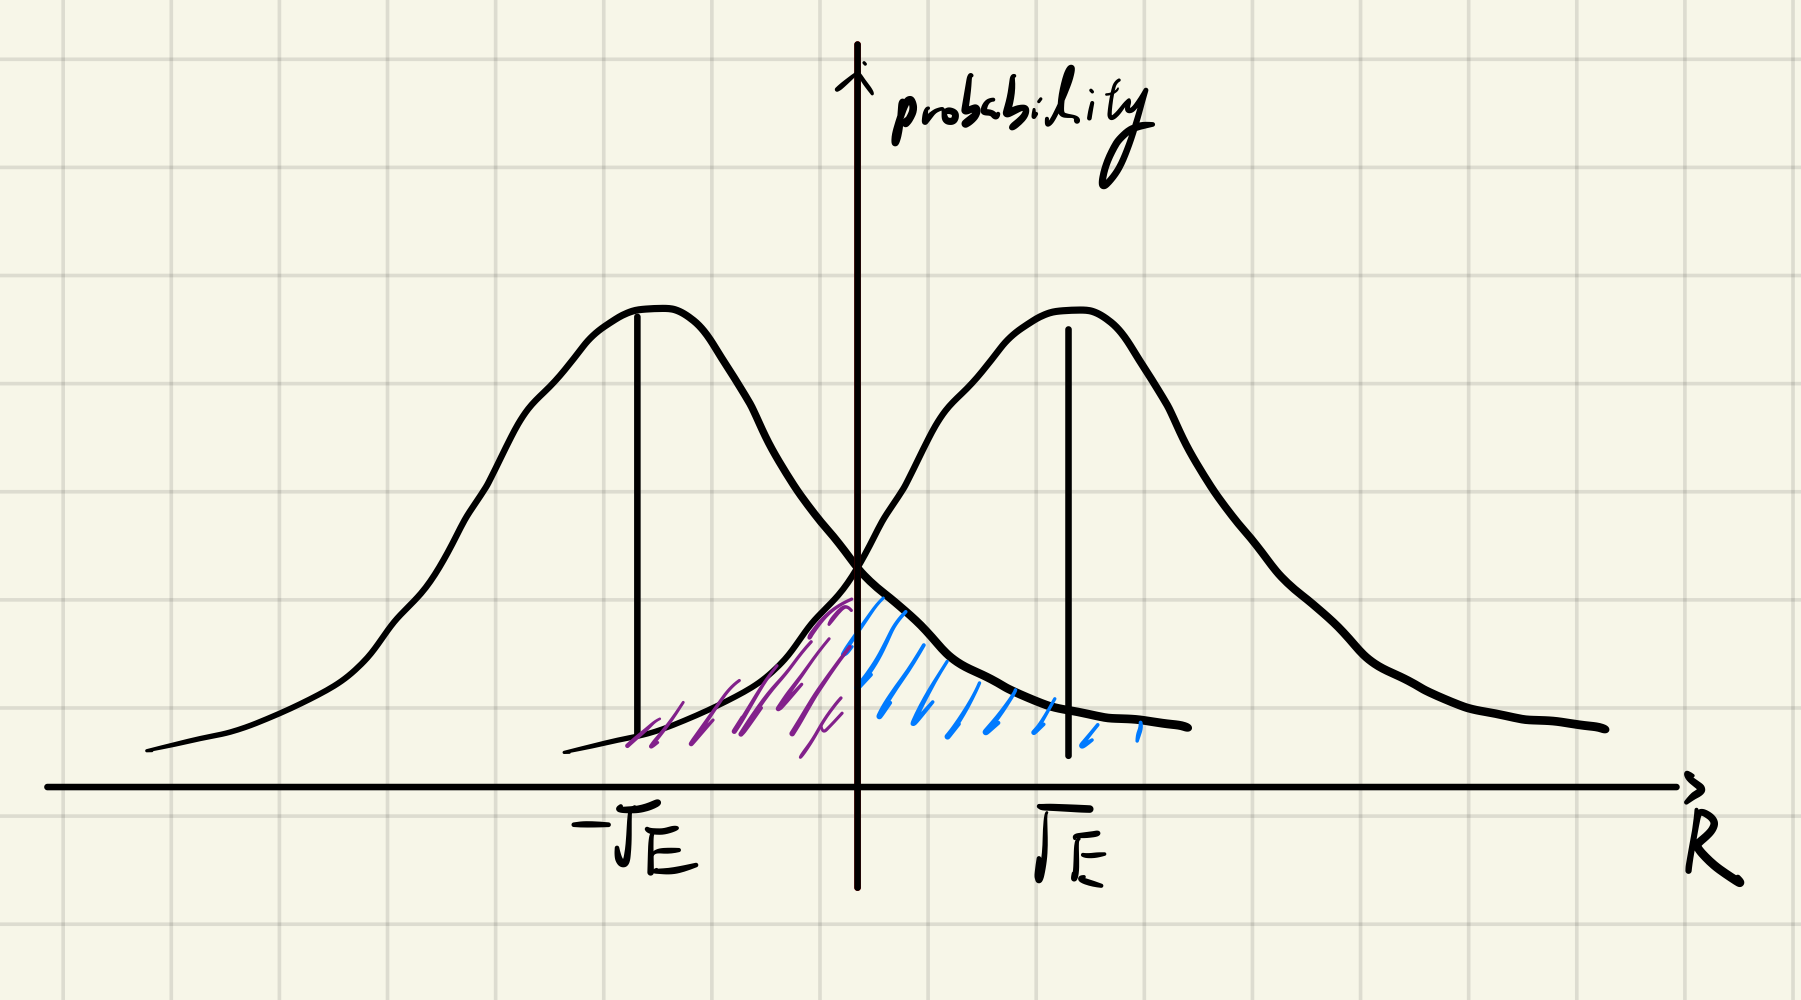
\includegraphics[width=0.5\textwidth]{./Figures/BPSK.png}
    \caption*{receiving signal under the effect of noise.}
\end{figure*}
If we assume that the receiving \(x = \hat{b} + w\) greater than zero is 1 and 0 otherwise, the question will \textbf{how do we calculate the blue/purple area?}
The blue area represent an error where 0 is recognized as 1.   
Qualitatively, we may skip a load of definition and conclude that the area of blue/purple is calculated as
\[
    \frac{1}{2}\int_{\sqrt{\frac{E_0}{N_0}}}^{\infty} \frac{2}{\sqrt{\pi } }e^{-u^2}du  
\] 
As we know that this integral is hard to compute, so we want an estimation. 
This will become a easier problem if we consider \(X\) with p.d.f \(f(x) = \frac{2}{\sqrt{pi} } e^{-x^2}, x \geq  0\), and thus \(E[X] = \frac{e^{-x^2}}{\sqrt{\pi } }\)      
Hence, we may apply Markov inequality to get 
\[
    P (X \geq c ) \leq \frac{E[X]}{c} = \frac{e^{-c^2}}{c\sqrt{\pi } }, 
\] 
where \(c = \sqrt{ \frac{E_0}{N_0}}\). 
\subsubsection*{Chebyshev inequality}
The last inequality we will introduce here is Chebyshev inequality.
\begin{note}[Chebyshev inequality]
   Let X be \textbf{any} r.v. Then for \textbf{any} \(t > 0\),
   \[
    P(|X - E[X]| \geq t) \leq \frac{\text{Var} (X)}{t^2}
   \]  
\end{note}
It is a direct application of Markov inequality as \( P(|X - E[X]| \geq t) = P(|X - E[X]|^2 \geq t^2) \), and \(E[(X - E[X])^2] = Var(X)\) 
 

\subsection{Converge in probability}
If we say \textbf{ \(X_n \to c\) in probability}, we means the sequence of random varaibles \((X_i)_{i=1}^\infty\) will eventually be really close to \(c\) in a way that
those \(\omega \) that does not map close to \(c\) will eventually has measure zero. 
\[
    \lim\limits_{n \to \infty} P(|X_n -c| \geq \epsilon  ) = 0
\]    
for every \(\epsilon >0\). 
\subsection{The weak law of large number (WLLN)}
Direct application of Chebyshev inequality. If we consider \textbf{i.i.d} \((X_i)_{i=1}^{\infty} \), then the mean \(\bar{X}_n\) will be really close to the expectation of \(X_1\), \(E[X_1]\). 
In formal expression we write \(\bar{X}_n \to E[X_1]\) in probability. 

\textbf{Tips when using WLLN:}\\
The key to this type of problem is to show that the variance will have \textbf{limit 0} as n grows.  